\chapter{Технологическая часть}

    В разделе представлены средства разработки программного обеспечения и детали реализации.
    
    \section{Средства реализация}
	Для реализации программного обеспечения выбран язык С++ \cite{cpp}. Выбор обуславливается тем, что язык представляет весь необходимый для решения поставленной задачи функционал.      

        Для создания пользовательского интерфейса ПО был использован фреймворк QT\cite{qt}. Фреймворк содержит объекты, позволяющие напрямую работать с пикселями изображения, а  так же возможности создания интерактивных пользовательских интерфейсов.
        
        Для сборки программного обеспечения использовался инструмент QMake\cite{qt}.
        
        В качестве среды разработки была выбрана среда разработки QtCreator\cite{qt}.

\section{Используемые классы}

Используемые классы представлены на рисунке \ref{img/uml1}. Класс BaseObject является базовым для объектов сцены, класс Camera содержит описание наблюдателя, класс Scene хранит объекты сцены, наблюдателя и фотонные карты прямого и непрямого освещения сцены. В классе Вrawer реализованы функции, отвечающие за построения изображения сцены.

\begin{figure}[H]
		\center{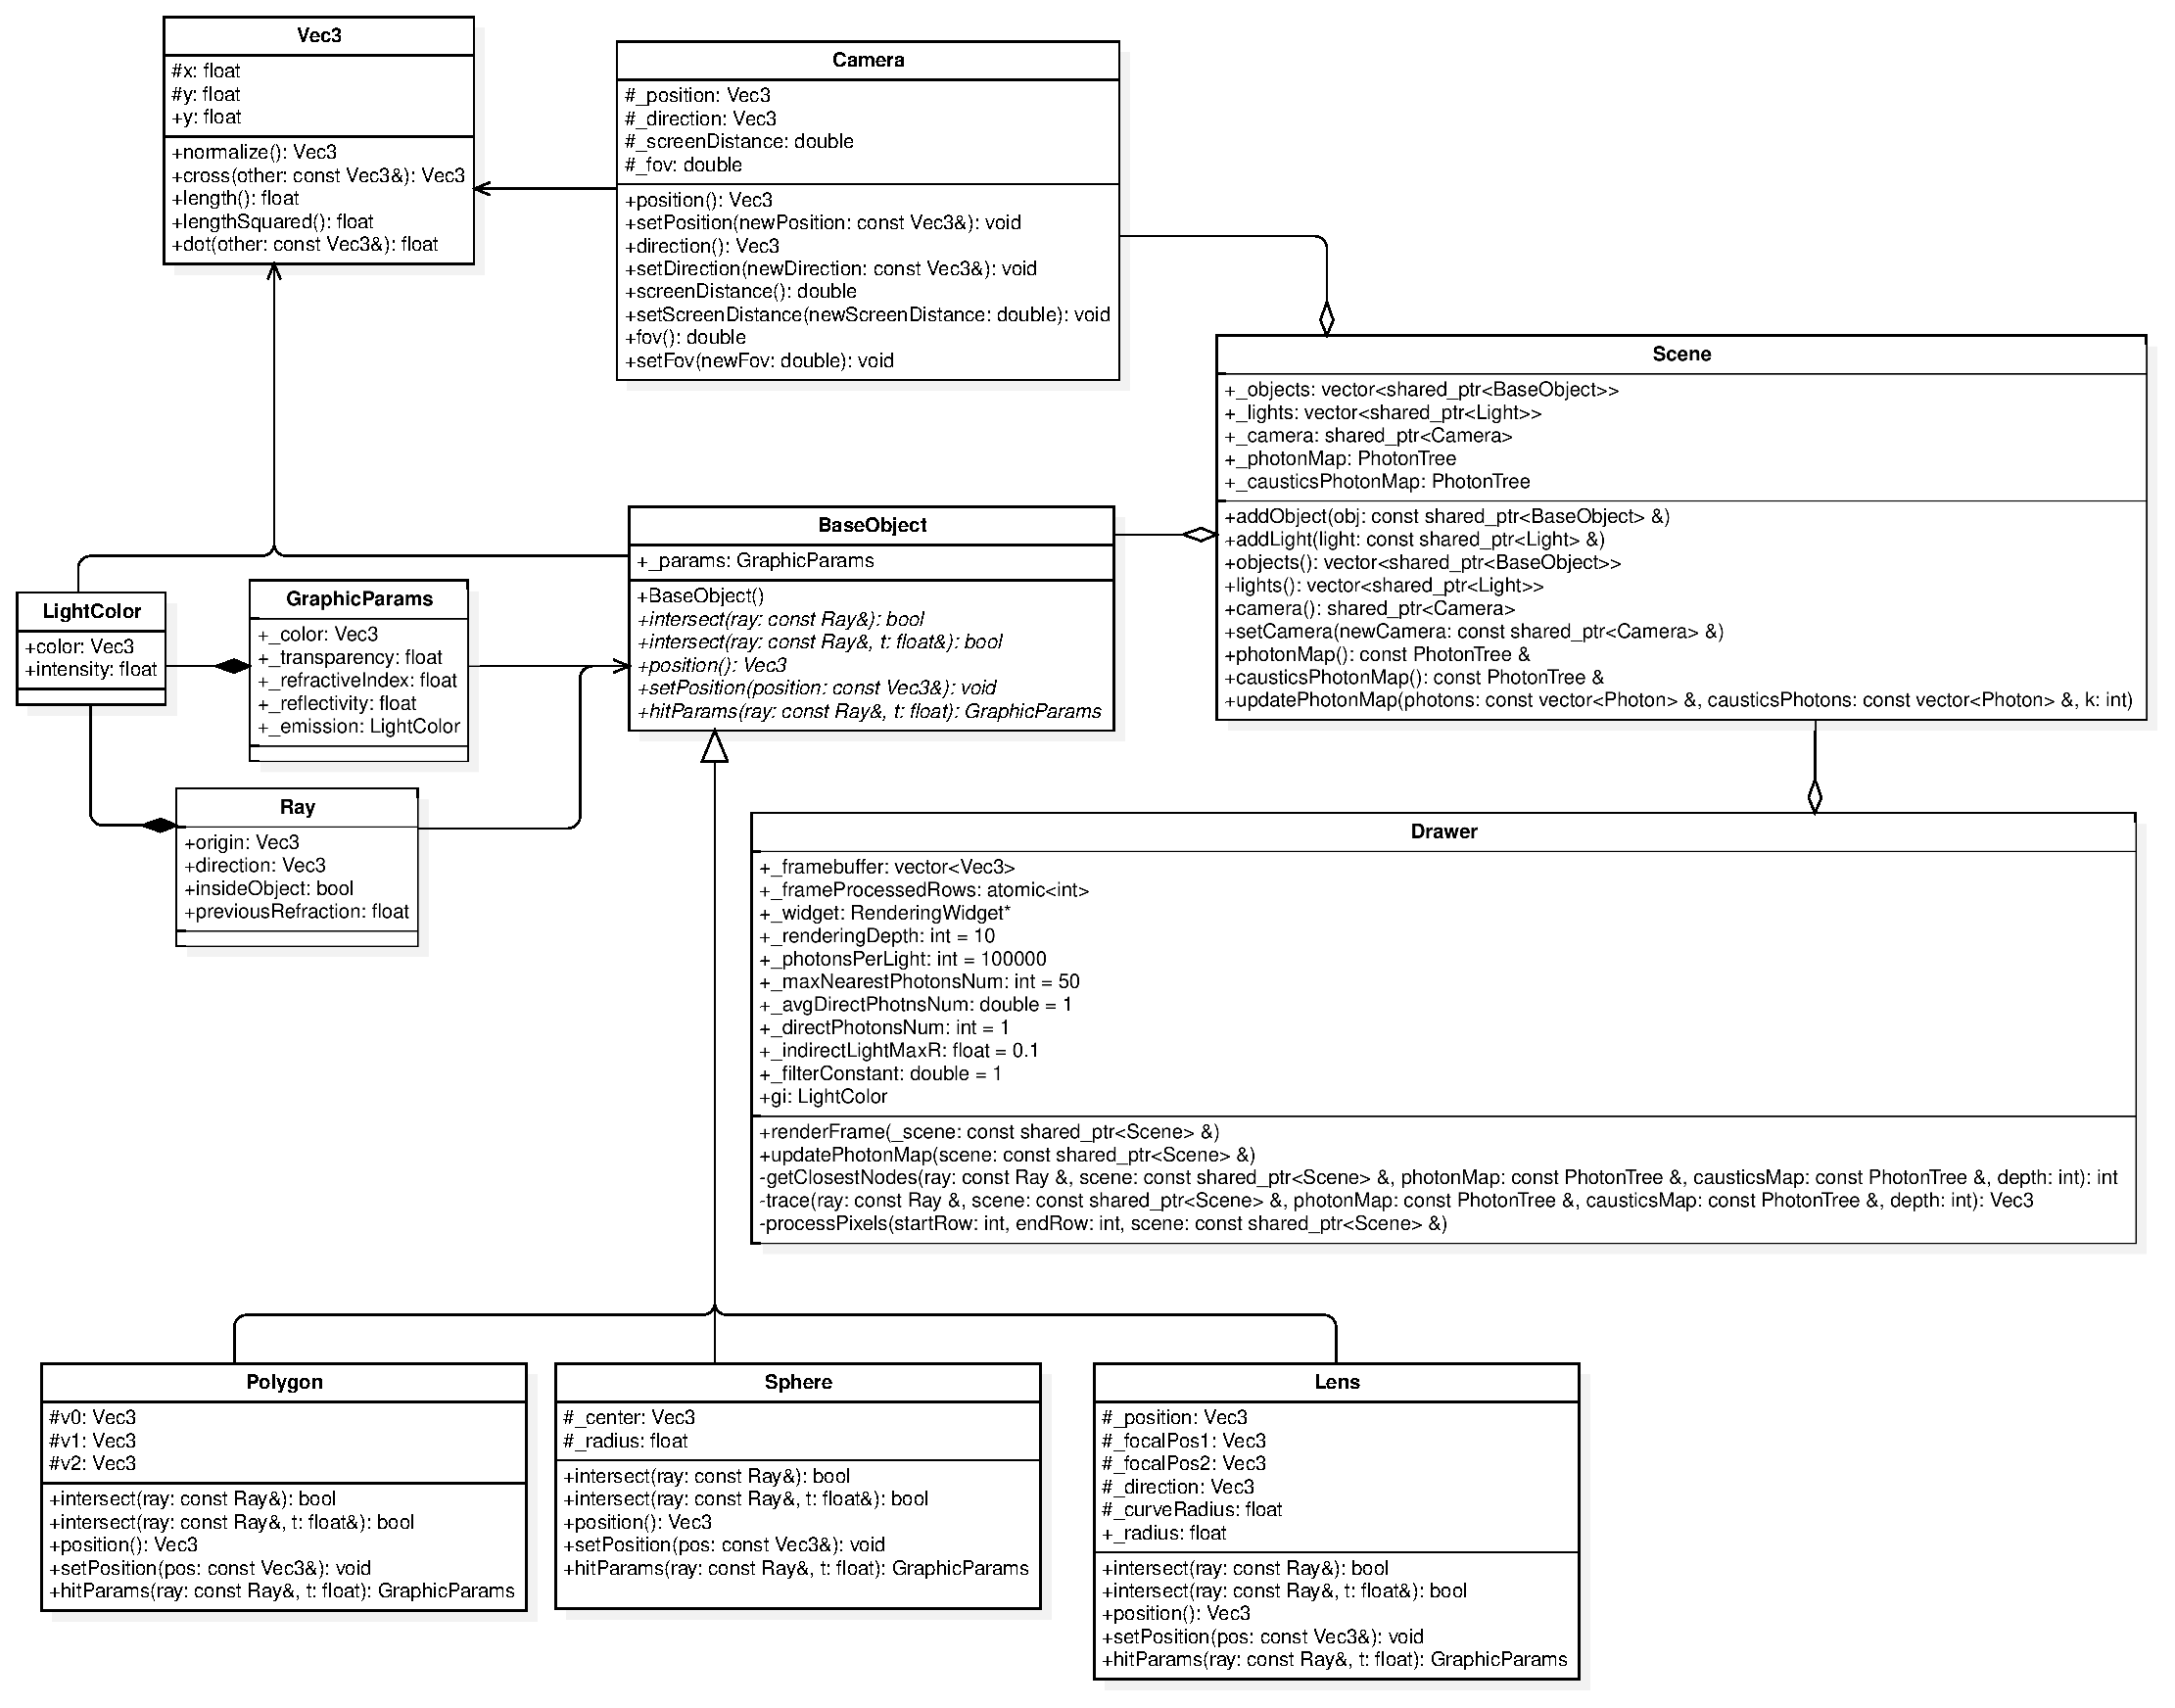
\includegraphics[width=\textwidth, height=210mm, width=170mm, keepaspectratio]{img/uml_1.eps}}
		\caption{UML диаграмма используемых классов}
		\label{img/uml1}
\end{figure}

    \section{Пользовательский интерфейс}
    
        Интерфейс реализуемого ПО представлен на рисунках \ref{img/ui_render} – \ref{img/ui}.
        

На рисунке \ref{img/ui_render} представлены параметры отрисовки, пользователь может задать число фотонов, испускаемых каждым источником света, радиус сбора освещенности и коснтанту фильтра, который используется в алгоритме сбора освещенности от ближайших фотонов, определяя влияния расстояния от точки до фотона на освещенность от этого фотона.
\begin{figure}[H]
		\center{\includegraphics[width=\textwidth, height=210mm, width=170mm, keepaspectratio]{img/ui_render.png}}
		\caption{Виджет параметров отрисовки}
		\label{img/ui_render}
\end{figure}
     
    На рисунке \ref{img/ui_camera} представлены параметры наблюдателя. Пользователь может задать положения камеры, направление ее взгляда и угол обзора.
\begin{figure}[H]
		\center{\includegraphics[width=\textwidth, height=210mm, width=170mm, keepaspectratio]{img/ui_camera.png}}
		\caption{Виджет параметров камеры}
		\label{img/ui_camera}
\end{figure}

На рисунке \ref{img/ui_sphere} представлены параметры сферы на сцене. Пользователь может определить положение, радиус, прозрачность, зеркальность, коэффициент преломления, цвет поверхности сферы, цвет и интенсивность излучения сферы.
\begin{figure}[H]
		\center{\includegraphics[width=\textwidth, height=210mm, width=170mm, keepaspectratio]{img/ui_sphere.png}}
		\caption{Виджет параметров сферы}
		\label{img/ui_sphere}
\end{figure}

На рисунке \ref{img/ui_polygon} представлены параметры треугольного полигона. Есть возможность задать положение трех его точек и графические параметры.
\begin{figure}[H]
		\center{\includegraphics[width=\textwidth, height=210mm, width=170mm, keepaspectratio]{img/ui_polygon.png}}
		\caption{Виджет параметров полигона}
		\label{img/ui_polygon}
\end{figure}

На рисунке \ref{img/ui_lens} представлены параметры линзы, имеется возможность изменить радиус кривизны, общий радиус, графические параметры и положение в пространстве.
\begin{figure}[H]
		\center{\includegraphics[width=\textwidth, height=210mm, width=170mm, keepaspectratio]{img/ui_lens.png}}
		\caption{Виджет параметров линзы}
		\label{img/ui_lens}
\end{figure}
        
На рисунке \ref{img/ui} представлен пример работы программы с несколькими прозрачными объектами.
\begin{figure}[H]
		\center{\includegraphics[width=\textwidth, height=210mm, width=170mm, keepaspectratio]{img/ui.png}}
		\caption{Пример работы программы}
		\label{img/ui}
\end{figure}
    
    \section{Вывод}

        В разделе были представлены средства разработки программного обеспечения, детали реализации, пользовательский интерфейс. Также были проедемонстрированы примеры работы программы.